In this section, we construct an special domain in the Euclidean plane, and then define a new model for hyperbolic plane based on this domain.
We show that this model is isometric to the Poincar\'e disk model. Finally, we provide two ways to construct the order-4 apeirogonal tiling of the hyperbolic plane.
We also defined three scalar fields $X, Y, L$ on the hyperbolic plane which will be used in the next section.

\subsection{The order-4 Cayley tree $T$}\label{sec:tree}

\begin{figure}
    \centering
    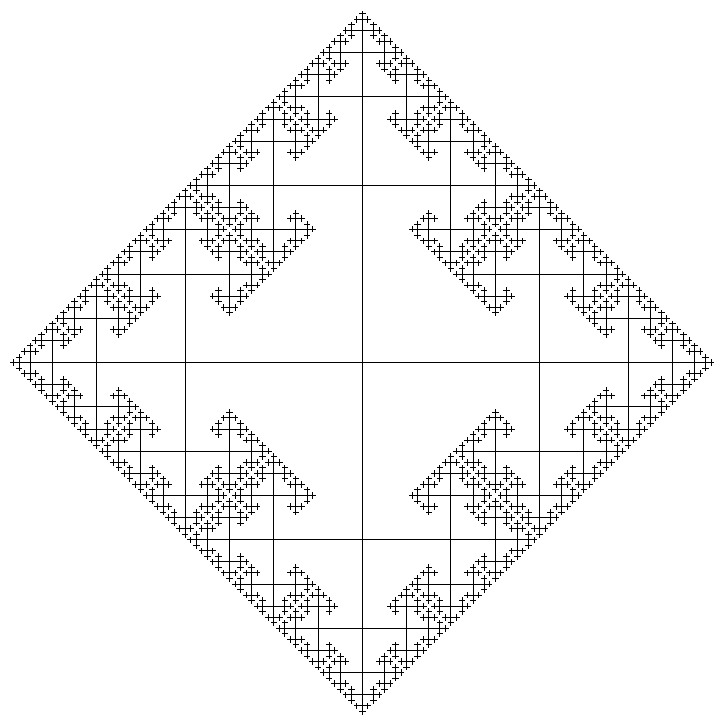
\includegraphics[width=0.6\textwidth]{images/cayley4}
    \caption{The order-4 Cayley tree}
\end{figure}


\subsection{A domain construction based on $T$}\label{sec:domain}

Cut and glue

We define a domain $D$ in the Euclidean plane as follows. Let $D$ be the union of the following regions:

\begin{figure}
    \centering
    
\includegraphics[width=0.2\textwidth]{images/cayley-tree-4-border-2}
    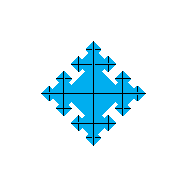
\includegraphics[width=0.2\textwidth]{images/cayley-tree-4-border-3}
    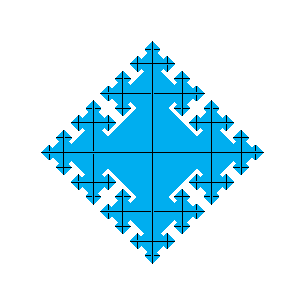
\includegraphics[width=0.2\textwidth]{images/cayley-tree-4-border-4}
    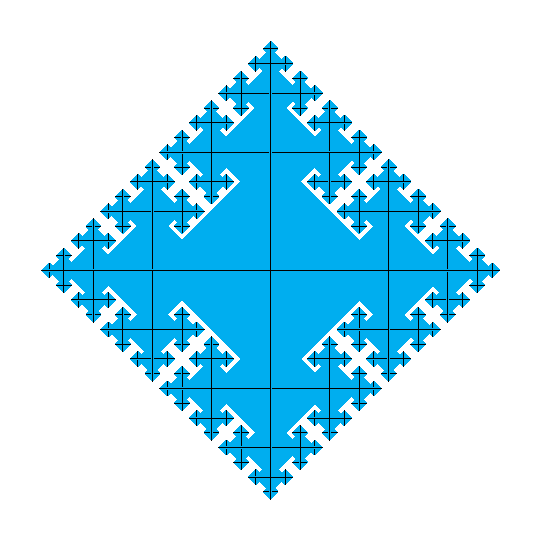
\includegraphics[width=0.2\textwidth]{images/cayley-tree-4-border-5}
    \caption{Construction steps 2, 3, 4, and 5 of the tree $T$ and the domain $D$}
\end{figure}

\subsection{$\mathcal{L}_1$ distance and functions $L, X, Y$ }\label{sec:fields}

\subsection{Cayley model of the hyperbloic plane $\mathbf{H}_2$}\label{sec:model}

\subsection{Order-4 apeirogonal tiling}\label{sec:tilling}

